\section{Sprint 2}

In this sprint we got a huge scope change. The reason for this is that we got a clue that our original plan with Qualisys and an external flight controller has to high latency. We will maybe not be able to stabilize the quadrotor using this method. Since our main goal with this project is to compare a fixed pitch with a variable pitch, and to see how the stability and performance differs, we will not get a reliable result. We therefore built a test rig with one fixed pitch rotor to see how well we are able to stabilize the rotor. From this test we can also measure the latency and get to know how the PID-controller works. We can also experiment with closed-loop control. 

\begin{figure}[h]
        \centering
        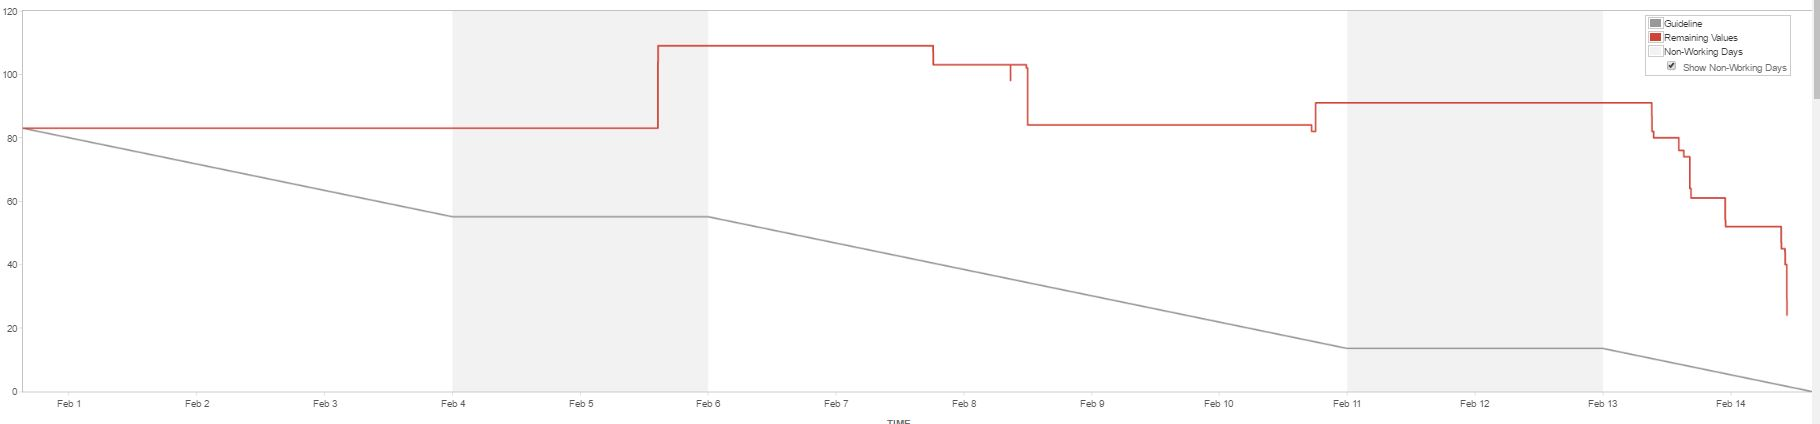
\includegraphics[width = 0.35\textwidth]{VAPIQ-PICTURES//SprintBD2.png}
        \\[2.0 cm] 
    \end{figure}            

